\documentclass{beamer}

\newcommand{\delim}{\line(1,0){290}}
\newcommand{\ssiz}{\scriptsize}

\usepackage{multicol}

%\setbeamercolor{cordotitulo}{bg=green!30!black,fg=white}
\useinnertheme{rounded}
\setbeamercolor{structure}{fg=teal!80!blue}
%\useoutertheme{smoothbars}
%\useoutertheme{shadow}
\useoutertheme[height=1 cm,width=1.5 cm]{sidebar}
%\usecolortheme{crane}
%\setbeamerfont{frametitle}{shape=\itshape}
\setbeamercolor{palette primary}{bg=teal!80!blue,fg=white}
\setbeamercolor{palette secondary}{bg=white,fg=white} %cor do logo
\setbeamercolor{palette tertiary}{bg=blue!70!black,fg=white}
\setbeamercolor{palette quaternary}{bg=white,fg=teal!80!blue}
\setbeamercolor{sidebar}{bg=teal!80!blue}
%\setbeamercolor{palette sidebar primary}{bg=red,fg=black}
%\setbeamercolor{palette sidebar secondary}{bg=red,fg=black}
\setbeamercolor{palette sidebar tertiary}{fg=white} %Autor no sidebar
\setbeamercolor{palette sidebar quaternary}{fg=white} %Titulo no sidebar
\setbeamercolor{section in sidebar}{fg=teal!80!blue,bg=white} %A cor naum
\setbeamercolor{subsection in sidebar}{fg=teal!80!blue,bg=white} %A cor naum
%ativa parece ser uma media das duas
%\setbeamercolor{section in sidebar current}{fg=red}
\setbeamercolor{frametitle}{fg=white,bg=teal!80!blue} %mudar
%fg aqui
\setbeamercolor{title}{bg=teal!80!blue,fg=white}
\setbeamerfont{title}{series=\bf}
\setbeamercolor{author}{bg=teal!80!blue,fg=white}
\setbeamerfont{author}{series=\bf}
\setbeamercolor{normal text}{bg=white,fg=teal!50!black}
\logo{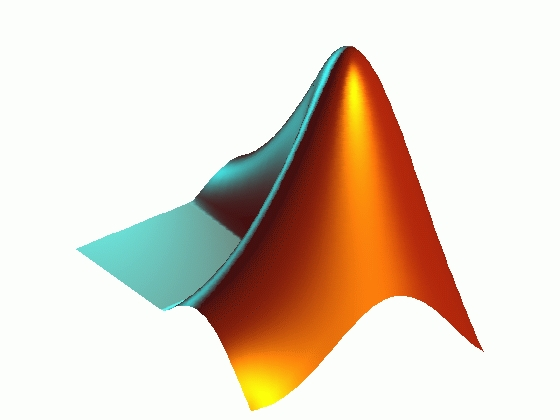
\includegraphics[scale=0.06]{matlab_logo.jpg}}

\title{Introdu\c{c}\~ao ao MatLab \\ Aula 1}
\author{Abel Siqueira \\ Kally Chung}
\date{}

\begin{document}

\frame{\titlepage}

\section[Introdu\c{c}\~ao]{}
\frame
{
  \frametitle{Introdu\c{c}\~ao}

  O Matlab \'e uma ferramenta poderosa com v\'arias vantagens:

  \begin{itemize}
  \item<2-> O Matlab \'e uma linguagem de alto n\'ivel especializada em vetores e matrizes.
  \item<3-> O Matlab cont\'em uma extensa biblioteca de fun\c{c}\~oes, programadas em C e Fortran.
  \item<4-> O Matlab facilita as opera\c{c}\~oes.
  \item<5-> No Matlab tamb\'em se pode programar.
  \item<6-> O Matlab cont\'em um sistema de ajuda muito forte.
  \end{itemize}
}
\frame
{
  \frametitle{Introdu\c{c}\~ao}

  No entanto, o Matlab tamb\'em tem algumas desvantagens:

  \begin{itemize}
  \item<2-> Por ser de alto n\'ivel, o Matlab n\~ao \'e t\~ao r\'apido quanto outras linguagens.
  \item<3-> O Matlab n\~ao \'e uma linguagem em si, e sim um programa, e al\'em disso, \'e pago.
  \item<4-> O Matlab gera uma falsa impress\~ao de que tudo \'e f\'acil.
  \end{itemize}

}
\subsection[\'Area de Trabalho]{}
\frame
{
  \frametitle{\'Area de Trabalho}

  A seguinte figura mostra a \'area de trabalho do Matlab.

  \begin{center}
  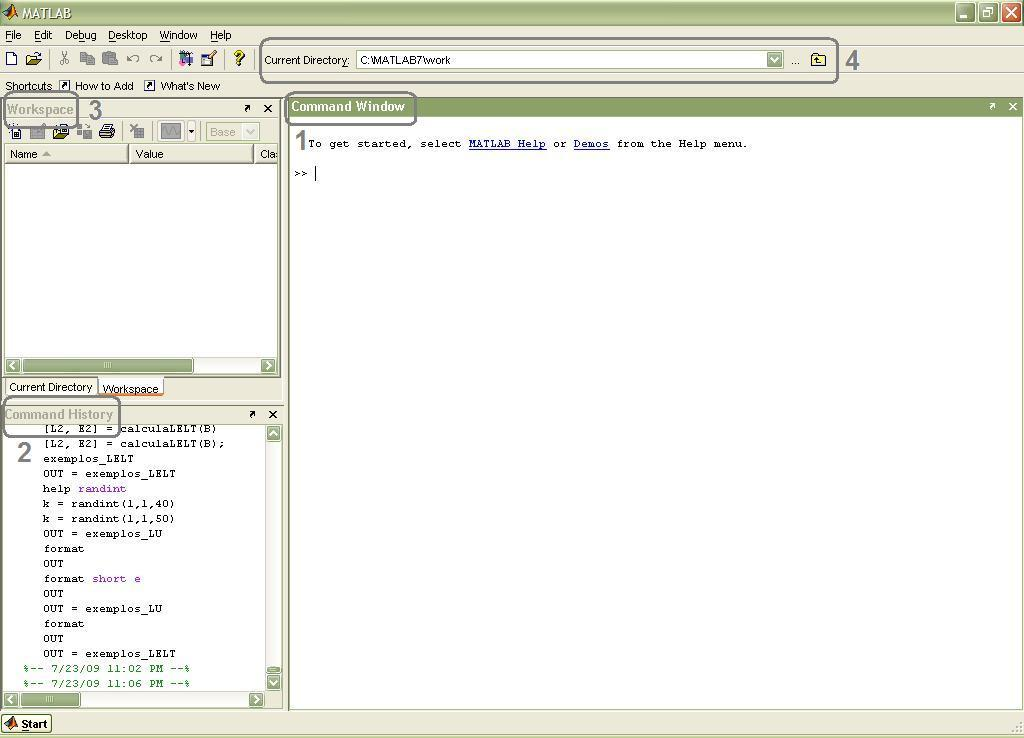
\includegraphics[scale=0.35]{figura2.jpg}
  \end{center}

}
\begin{frame}
 \frametitle{\'Area de Trabalho}

 \begin{itemize}
 \item<1-> A Janela de Comandos, ou Command Window, \'e a parte principal do Matlab. Nessa janela que escreveremos os comandos do programa.
 \item<2-> O Hist\'oricos de Comandos, ou Command History, \'e a janela onde aparecem os comandos digitados anteriormente.
 \item<3-> O Espa\c{c}o de Trabalho, ou Workspace, mostra as vari\'aveis que criamos.
  \item<4-> O Diret\'orio Atual, ou Current Directory, mostra o diret\'orio que o Matlab est\'a acessando atualmente. S\'o podemos chamar programas que estejam nesse diret\'orio.
 \end{itemize}
\end{frame}

\subsection[Opera\c{c}\~oes B\'asicas]{}
\frame
{
\frametitle{Opera\c{c}\~oes B\'asicas}

O Matlab permite as seguintes opera\c{c}\~oes aritm\'eticas elementares: {\tt +,
-, *, /, \textbackslash,  \textasciicircum}.
\pause

\begin{center}
\begin{tabular}{|c|c|}
\hline
Opera\c{c}\~ao & Exemplo \\ \hline
{\tt +} & {\tt 2.2 + 5} \\ \hline
{\tt -} & {\tt 23.7 - 32.99} \\ \hline
{\tt *} & {\tt 2001*1002} \\ \hline
{\tt /} ou \textbackslash & {\tt 501/41} ou 41\textbackslash501 \\ \hline
{\tt \textasciicircum} & {\tt 23\textasciicircum(5.3)} \\ \hline
\end{tabular}
\end{center}

}

\begin{frame}[fragile]
 \frametitle{Opera\c{c}\~oes B\'asicas}

Na Janela de Comando, fazemos
\pause
\delim
\begin{center}
\begin{minipage}{4 cm}
\begin{verbatim}
>> 5*2 + 4*0.25
ans =
    11
\end{verbatim}
\end{minipage}
\begin{minipage}{4 cm}
\begin{verbatim}
>> 2^(-10)
ans =
     9.7656e-004
\end{verbatim}
\end{minipage}
\end{center}
\delim
\pause

\begin{center}
\begin{minipage}{4 cm}
\begin{verbatim}
>> 1/3
ans =
     0.3333
\end{verbatim}
\end{minipage}
\begin{minipage}{4 cm}
\begin{verbatim}
>> 2/3
ans =
     0.6667
\end{verbatim}
\end{minipage}
\end{center}

\end{frame}

\subsection[Elementos B\'asicos]{}

\begin{frame}[fragile]
  \frametitle{Vari\'aveis}

  \begin{itemize}
  \item<1-> Note que, nos exemplos anteriores, apareceram os nomes {\tt ans}. {\tt ans} \'e uma vari\'avel criada pelo Matlab.

  \item<2-> Podemos criar outras vari\'aveis escrevendo {\tt <nome\_da\_vari\'avel> = <senten\c{c}a>}. O nome da vari\'avel pode conter letras, num\'eros e \_,mas n\~ao pode ter pontua\c{c}\~ao, acentua\c{c}\~ao e diferecia mai\'usculas e min\'usculas. Tamb\'em deve come\c{c}ar com uma letra.
  \end{itemize}
  \pause \pause
  \delim
  \begin{center}
  \begin{minipage}{4 cm}
  \begin{verbatim}
>> soma = 2 + 5
soma =
     7
  \end{verbatim}
  \end{minipage}
  \begin{minipage}{4 cm}
  \begin{verbatim}
>> mult = 4*3
soma =
     12
  \end{verbatim}
  \end{minipage}

  \begin{minipage}{4 cm}
  \begin{verbatim}
>> mult - soma
ans =
     5
  \end{verbatim}
  \end{minipage}
  \end{center}

\end{frame}

\begin{frame}

\frametitle{Vari\'aveis}

\begin{itemize}
\item<1-> Para visualizar as vari\'aveis que voc\^e est\'a atualmente utilizando, use o comando {\tt who}.
\item<2-> Para visualizar as vari\'aveis, com dimens\~ao e tipo, use o comando {\tt whos}.
\item<3-> Para apagar alguma vari\'avel do sistema utilize {\tt clear <nome\_da\_vari\'avel>}.
\item<4-> Para apagar todas as vari\'aveis utilize {\tt clear all}.
\item<5-> Para visualizar o valor de uma vari\'avel, utilize {\tt disp(<variavel>)} ou simplesmente {\tt <variavel>}.
\end{itemize}

\pause \pause \pause \pause \pause
Os seguintes nomes n\~ao podem ser utilizados como nomes de vari\'aveis:
{\tt \begin{center} \scriptsize
\begin{tabular}{|c|c|c|c|c|c|}
\hline
for & end & if & while & function & return \\ \hline
elseif & case & otherwise & switch & continue & else \\ \hline
try & catch & global & persistent & break & \\ \hline
\end{tabular}
\end{center}}
\end{frame}

\begin{frame}[fragile]
\frametitle{Vari\'aveis}

O Matlab cont\'em as seguintes vari\'aveis pr\'e-determinadas:

\begin{center}
\begin{tabular}{|c|c|}
\hline
{\tt pi} & $\pi = 3.14159265358979...$ \\ \hline
{\tt inf} & $\infty$, infinito. \\ \hline
{\tt NaN} & N\~ao \'e um n\'umero ({\it Not a Number}). \\ \hline
{\tt i} ou {\tt j} & Valor complexo para $\sqrt{-1}$. \\ \hline
\end{tabular}
\end{center}
\pause
Para escrever coment\'arios no Matlab, utilize {\tt \%}.{\small
\begin{verbatim}
>> 22.5 - 7.3 %Este eh um comentario
ans =
     15.2
>> 5 + %3
??? 5 + %3
          |
Error: Incomplete or misformed expression or statement.
\end{verbatim}
}
\end{frame}
\begin{frame}[fragile]

\frametitle{Tipos de Dados}

Al\'em de suportar os n\'umeros reais, o Matlab tamb\'em suporta os n\'umeros complexos e strings. Para escrever n\'umeros complexos utilizamos {\tt i} ou {\tt j}:
\pause
\begin{verbatim}
>> (2 + i)*i
     ans = -1.0000 + 2.0000i
>> 2 + 5i - (4 + 3j)
     ans = -2.0000 + 2.0000i
\end{verbatim}

\pause

Para escrever strings, utilizamos aspas simples:

\begin{verbatim}
>> `Matlab'
ans =
     Matlab
\end{verbatim}

\end{frame}
\begin{frame}[fragile]

\frametitle{Formatos de Exibi\c{c}\~ao de N\'umeros}
{\small
No Matlab, normalmente vemos os n\'umeros da forma com quatro casas decimais e nota\c{c}\~ao cient\'ifica quando necess\'ario. Mas existem outras formata\c{c}\~oes poss\'iveis. Para mudar a formata\c{c}\~ao utilizamos o comando {\tt format}:
}
\pause

{\scriptsize \tt
\begin{center}
\begin{tabular}{|l|l|l|}
\hline
{\normalfont Comando} & $\pi$ & $2^{-10}$ \\ \hline
{\tt format short} & 3.1416 & 9.7656e-004 \\ \hline
{\tt format long} & 3.14159265358979 & 9.765625000000000e-004 \\ \hline
{\tt format short e} & {\tt 3.1416e+000} & 9.7656e-004 \\ \hline
{\tt format long e} & 3.141592653589793e+000 & 9.765625000000000e-004 \\ \hline
{\tt format short g} & 3.1416 & 0.00097656 \\ \hline
{\tt format long g} & 3.14159265358979 & 0.0009765625 \\ \hline
{\tt format bank} & 3.14 & 0.00 \\ \hline
\end{tabular}
\end{center}
}
\pause

{\scriptsize
Para que o Matlab n\~ao escreva o resultado do que voc\^e estiver fazendo, utilize {\tt ;}
\pause

\begin{center}
\begin{minipage}{4 cm}
\begin{verbatim}
>> soma = 10 + 5
soma =
     15
\end{verbatim}
\end{minipage}
\begin{minipage}{4 cm}
\begin{verbatim}
>> soma = 10 + 5;
>> soma
soma =
     15
\end{verbatim}
\end{minipage}
\end{center}
}

\end{frame}

\begin{frame}[fragile]
 \frametitle{Fun\c{c}\~oes Matem\'aticas}

A seguir est\~ao algumas das fun\c{c}\~oes matem\'aticas do Matlab. Para utiliz\'a-las basta escrever o nome da fun\c{c}\~ao e entre par\^enteses o argumento.

{\scriptsize \tt
\begin{center}
\begin{tabular}{|c|c|c|c|c|c|c|c|}
\hline
sin  & cos  & tan   & sec  & csc   & cot  & sinh & cosh \\ \hline
asin & acos & atan  & abs  & rem   & real & imag & sign \\ \hline
exp  & log  & log10 & sqrt & floor & ceil & round & fix \\ \hline
deg2rad & rad2deg & num2str & conj & & & & \\ \hline
\end{tabular}
\end{center}
}
\pause
Exemplo:
{\ssiz
\begin{center}
\begin{minipage}{4 cm}
\begin{verbatim}
>> sin(pi/4)
ans =
     0.7071
>> abs(3+4*i)
ans =
     5
\end{verbatim}
\end{minipage}
\begin{minipage}{4 cm}
\begin{verbatim}
>> ceil(exp(1))
ans =
     3
>> conj(3+4*i)
ans =
   3.0000 - 4.0000i
\end{verbatim}
\end{minipage}
\end{center}
}

\end{frame}

\section[Exerc\'icios]{}

\begin{frame}
\frametitle{Exerc\'icios}

\begin{enumerate}
\item Crie duas vari\'aveis, $x$ e $y$, sendo a primeira o seu RA, e a segunda seu RA escrito ao contr\'ario. Cria as vari\'aveis:
\begin{enumerate}
\item $S$ que guarde a soma de $x$ e $y$.
\item $M$ que guarde a multiplica\c{c}\~ao de $x$ e $y$.
\item $E$ que guarde a exponencial de $S$.
\item $L$ que guarde o logaritmo natural de $M$.
\end{enumerate}
\item Calcule as seguintes express\~oes:
\begin{enumerate}
\begin{multicols}{2}
\item $\dfrac{\sin(\pi/12)+\cos(\arctan(1))}{e^2-\ln(2)}$
\item $\dfrac{\sqrt{10}+10^2}{\sqrt{\sin^2(5\pi/7)}}$
\end{multicols}
\end{enumerate}
\item Crie a vari\'avel $z = \dfrac{1+\sqrt{5}}{2}$. Calcule $z^2-z-1$.
\end{enumerate}
\end{frame}


\end{document}